\section{Introduction}
	\subsection{Kinesin-1: Cell's workhorses}
		All life forms in our universe are made of cells. To understand the mechanisms in and between those elementary building blocks of life is a real fundamental aim of biology, biochemistry and biophysics. But understanding these tiny but really complex structures also means understanding thousands of finely tuned mechanisms that are essential for survival of a cell. One necessary condition for most of these processes is a \textit{directional} (not statistical!) motion of cell components. For example the segregation of chromosomes during cell division would not work with brownian motion alone. Fortunately there are so called \textit{motor proteins} as kinesin, dynesin and myosin that are responsible for these kinds of motion appearing in many transport-mechanisms.\\
		In the following experiment we will investigate \textit{kinesin-1}, a motor protein moving along \textit{microtubule} filaments. For that purpose we will measure their velocity and the mean run length. But at first some basic knowledge.\\
		\ \\
		\textbf{Microtubules} (MTs) are a component of the cytoskeleton that can be depicted with the "cell's highway" because they form basically the ground where the motorproteins can walk on. Their basic building blocks are the $\alpha-/\beta$-tubulin heterodimers that polymerise longitudinally in a periodic structure with a repeat-length of $8\ \unit{nm}$. They form a structure of hollow-cylinders having an outer diameter of $25\ \unit{nm}$. Because of the reversible binding and the hydrolysis of GTP(in figure \ref{int:MT} dyed red) by $\beta$-tubulin MTs show a highly dynamic growing behavior that is necessary to build those "roads" as flexible as possible. Later we have to surpress this effect. The directed motion on the MTs is enabled by the structural polarity of the tubulin-dimers. Figure \ref{int:MT} shows the strucuture of the MTs.\cite{PA}\\
		\begin{figure}[h]
		 			\centering
		 		   	\captionsetup{justification=raggedright, margin =4cm}            
		 		    	  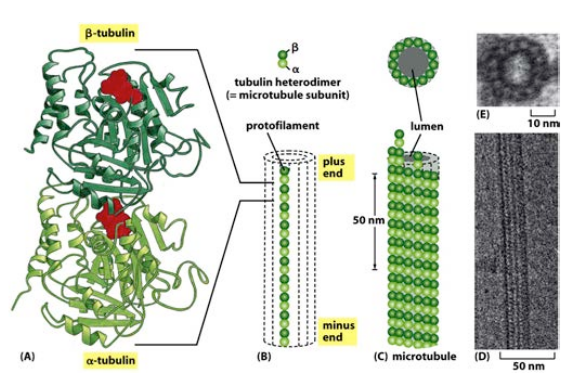
\includegraphics[scale=0.3]{pic/mt.png}
		 		    \caption{Structure of the microtubules\cite{PA}}
		 		   	\label{int:MT} 
		\end{figure}\\
		\textbf{Kinesin-1} is a motor-protein that moves along the MT transporting different types of cargo (e.g. vesicles, mitochrondria, chromosomes) in the cells. It consists of two identical subunits that are winded into each other. For the motion from the minus-end to the plus-end of the MTs it uses the strucutural polarity of the tubulin-subunits binding its motor domain just to the $\beta$-tubulin parts. So it moves in discrete steps of $\Delta x = 8\  \unit{nm}$ exerting a force of $F = 5\ \unit{pN}$ to the MT-surface powered by the hydrolisis of an ATP-molecule during each step. The ATP-hydrolysis leads to an energy-emission of $E_{ATP} = 101 \cdot 10^{-21}\ \unit{J}$ while the motorproteins do a work of $W_{MP} = F \cdot \Delta x = 4 \cdot 10^{-20}\ \unit{J}$. This means an efficiency of $\eta = W_{MP} / E_{ATP} = 39.60\ \unit{\%}$.\cite{PA} The mechanochemical cycle of kinesin-1 is visualised in Figure \ref{int:kinesin}:
		\begin{figure}[h]
				 			\centering
				 		   	\captionsetup{justification=centering}            
				 		    	  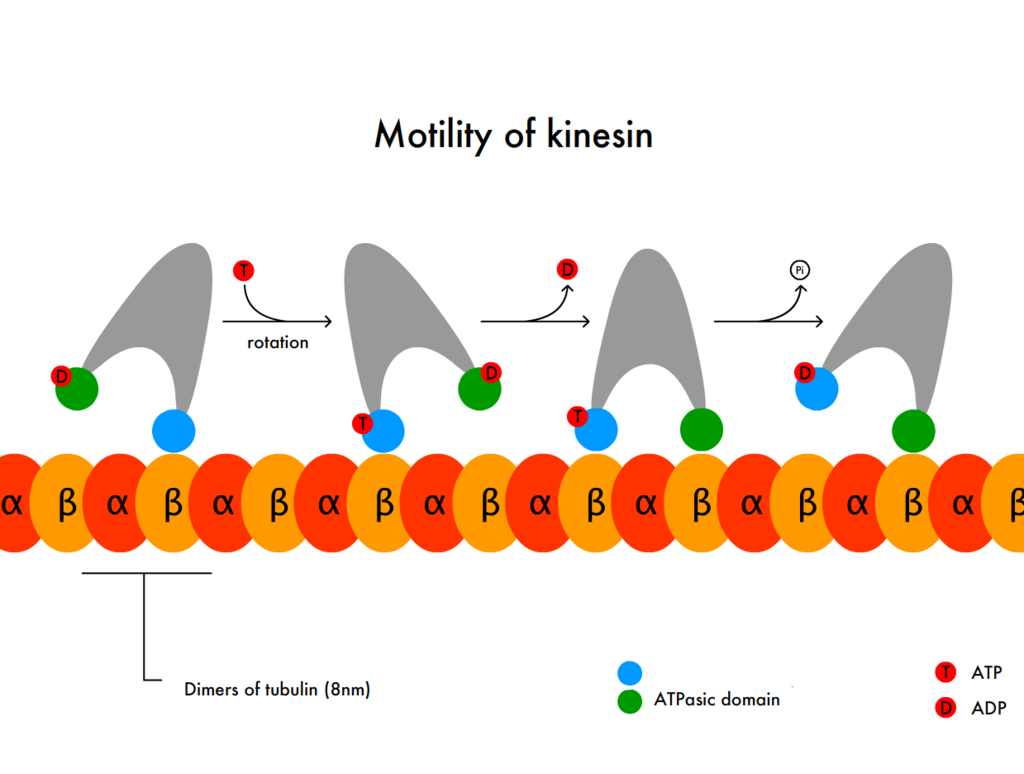
\includegraphics[scale=0.3]{pic/kinesin.png}
				 		    \caption{Mechanochemical cycle of Kinesin-1:\\ Absorbing of ATP, Emitting of ADP, ATP Hydrolysis\cite{wikiKinesin}}
				 		   	\label{int:kinesin} 
				\end{figure}\\
	\subsection{Fluorescence Microscopy}
       In fluorescence microscopy the emission of light by a marked assay is used. More accurate, an electron in an excited singlet state within a molecule is paired by the contrary spin to the second electron in the ground-state orbital. The return to the ground state is allowed by spin (pauli principle). This appears rapidly with an emission rate of about $\unit[10^8]{s^{-1}}$ by the emission of a photon.
        \subsubsection{Fluorescent markers}
            There are two types of fluorescent markers: intrinsic and extrinsic. The intrinsic ones appear naturally in the sample (for example chlorophyll). Extrinsic markers are added to the probes, when fluorescence does not appear naturally (e.g. flourescein).
            In a conjugated p-electron-system they have delocalized electrons. In this system, the first excitation energy of the molecule is comparatively low, so it can be stimulated by visible light.
            In this expermient, microtubules where marked with rhodamine and the motor proteins by green flourescence protein (GFP).
        \subsubsection{Total internal reflection Flourescence Mircroscopy}
            Total internal reflection fluorescence (TIRF) microscopy is used in this experiment. The base of this methodology is the total internal reflection. It can be detected when a beam of light travels from a medium with high refractive index to a medium with a low one under an angle bigger than the critical angle $\alpha_c$.
            Even though the beam is totally reflected an exponentially decaying field called the \textit{evanescent field} occurs. It reaches typically $\unit[100]{nm}$ into the medium with the lower refractive index.
            This distance is useful, because it naturally creates a way to limit the volume where flourophores get excited. In this way the noise lowering the contrast between the signals and the background is surpressed.
            
